% GW Pathfinder thesis - Tribhuwan University project-work format.
% Structure follows: https://www.overleaf.com/latex/templates/tribhuwan-university-project-work-template/kgqnczfcbjrr
%
% COMPILE WITH XeLaTeX (required for polyglossia + the Devanagari abstract).
% No LaTeX toolchain was available in the environment this was written in,
% so this has NOT been test-compiled - open it on Overleaf (where the
% reference template lives) and build once before relying on it.
%
% TODO markers throughout mark content that needs the student's/university's
% specific details (name, roll number, supervisor, board members, dates).
% Scientific content is drawn from docs/ and legs/*/docs/ where available.

\documentclass[12pt,a4paper,oneside]{report}

\usepackage{fontspec}
\usepackage{polyglossia}
\setmainlanguage{english}
\setotherlanguage{nepali}
% TODO: uncomment once a Devanagari-capable font is confirmed installed on
% the compiling machine (Overleaf has several preinstalled, e.g. below):
% \newfontfamily\devanagarifont{Noto Sans Devanagari}

\usepackage[a4paper,left=3.5cm,right=2.5cm,top=2.5cm,bottom=2.5cm]{geometry}
\usepackage{setspace}
\onehalfspacing

\usepackage{graphicx}
\usepackage{caption}
\usepackage{subcaption}
\usepackage{array}
\usepackage{float}
\usepackage{amsmath}
\usepackage{amssymb}
\usepackage{booktabs}
\usepackage{tabularx}
\usepackage{hyperref}
\hypersetup{colorlinks=true, linkcolor=black, citecolor=black, urlcolor=blue}
\usepackage{apacite}
\usepackage[acronym]{glossaries}
\makeglossaries
\usepackage{titlesec}

\counterwithin{figure}{chapter}
\counterwithin{table}{chapter}
\counterwithin{equation}{chapter}

% List of Acronyms and Abbreviations - add \newacronym entries as the thesis grows.
\newacronym{gw}{GW}{Gravitational Wave}
\newacronym{lvk}{LVK}{LIGO/Virgo/KAGRA}
\newacronym{gcn}{GCN}{General Coordinates Network}
\newacronym{snr}{SNR}{Signal-to-Noise Ratio}
\newacronym{far}{FAR}{False Alarm Rate}
\newacronym{bbh}{BBH}{Binary Black Hole}
\newacronym{bns}{BNS}{Binary Neutron Star}
\newacronym{nsbh}{NSBH}{Neutron Star-Black Hole}
\newacronym{gwtc}{GWTC}{Gravitational-Wave Transient Catalog}
\newacronym{gwosc}{GWOSC}{Gravitational Wave Open Science Center}
\newacronym{llm}{LLM}{Large Language Model}
\newacronym{loo}{LOO}{Leave-One-Out (cross-validation)}
\newacronym{mae}{MAE}{Mean Absolute Error}
\newacronym{rmse}{RMSE}{Root Mean Squared Error}


\title{Rapid Chirp-Mass Estimation and AI-Assisted Analysis of Gravitational-Wave GCN Circulars} % TODO: confirm final title with supervisor
\author{Swastika Yogi} % TODO: confirm exact name as it should appear

\begin{document}

\pagenumbering{roman}

% TODO: replace every bracketed placeholder with your actual institutional details.
\begin{titlepage}
    \centering
    \vspace*{1cm}
    {\large [UNIVERSITY NAME]} \\ % TODO
    {\large [FACULTY / INSTITUTE NAME]} \\ % TODO
    {\large [COLLEGE NAME]} \\ % TODO

    \vspace{2cm}
    {\Large \bfseries Rapid Chirp-Mass Estimation and AI-Assisted Analysis of \\ Gravitational-Wave GCN Circulars} \\ % TODO: confirm title
    \vspace{0.5cm}
    {\large A Project Report} \\

    \vspace{2cm}
    Submitted in partial fulfillment of the requirements for the degree of \\ % TODO: confirm exact wording your department uses
    {\bfseries [DEGREE TITLE]} \\ % TODO

    \vspace{2cm}
    {\large Submitted by:} \\
    {\bfseries Swastika Yogi} \\ % TODO
    {[ROLL NUMBER / SYMBOL NUMBER]} \\ % TODO

    \vspace{2cm}
    {\large [MONTH, YEAR]} % TODO

    \vfill
\end{titlepage}

% TODO: this page is signed by your supervisor - fill in once they've reviewed the final draft.
\chapter*{Recommendation}
\addcontentsline{toc}{chapter}{Recommendation}

This is to certify that this project work entitled \textbf{``Rapid Chirp-Mass Estimation and AI-Assisted Analysis of Gravitational-Wave GCN Circulars''} has been carried out by \textbf{Swastika Yogi} under my supervision. % TODO: confirm wording with supervisor
In my opinion, this report is in a form suitable for evaluation as partial fulfillment of the requirements for the degree stated on the title page.

\vspace{2cm}
\noindent
\begin{tabular}{@{}l}
\hrulefill \\
[SUPERVISOR NAME] \\ % TODO
[SUPERVISOR TITLE / DEPARTMENT] \\ % TODO
Date: \underline{\hspace{4cm}}
\end{tabular}

\chapter*{Declaration}
\addcontentsline{toc}{chapter}{Declaration}

I hereby declare that the work presented in this project report entitled \textbf{``Rapid Chirp-Mass Estimation and AI-Assisted Analysis of Gravitational-Wave GCN Circulars''} is my own original work, carried out under the supervision of [SUPERVISOR NAME], % TODO
and has not been submitted elsewhere for the award of any degree or diploma.
All sources of information have been acknowledged through appropriate citation.

\vspace{2cm}
\noindent
\begin{tabular}{@{}l}
\hrulefill \\
Swastika Yogi \\ % TODO
[ROLL NUMBER / SYMBOL NUMBER] \\ % TODO
Date: \underline{\hspace{4cm}}
\end{tabular}

% TODO: written/signed by the Head of Department or equivalent - fill in per your department's exact wording convention.
\chapter*{Letter of Forward}
\addcontentsline{toc}{chapter}{Letter of Forward}

[Department letterhead / forwarding statement per institutional format.] % TODO

\vspace{2cm}
\noindent
\begin{tabular}{@{}l}
\hrulefill \\
[HEAD OF DEPARTMENT NAME] \\ % TODO
[TITLE] \\ % TODO
Date: \underline{\hspace{4cm}}
\end{tabular}

% TODO: filled in after the defense/evaluation board - leave blank until then.
\chapter*{Board of Examination Certificate}
\addcontentsline{toc}{chapter}{Board of Examination Certificate}

This project report entitled \textbf{``Rapid Chirp-Mass Estimation and AI-Assisted Analysis of Gravitational-Wave GCN Circulars''}, submitted by \textbf{Swastika Yogi}, % TODO
has been examined and accepted as satisfying the project-work requirement for the degree of [DEGREE TITLE]. % TODO

\vspace{2cm}
\noindent
\begin{tabular}{@{}ll}
\hrulefill & \hrulefill \\
Internal Examiner & External Examiner \\ % TODO
[NAME] & [NAME] \\ % TODO
\end{tabular}

\vspace{1cm}
\noindent
\begin{tabular}{@{}l}
\hrulefill \\
[PROGRAM COORDINATOR / HOD] \\ % TODO
Date: \underline{\hspace{4cm}}
\end{tabular}

% TODO: personal - write this yourself. A placeholder structure is given below.
\chapter*{Acknowledgement}
\addcontentsline{toc}{chapter}{Acknowledgement}

I would like to express my sincere gratitude to [SUPERVISOR NAME] for their guidance and support throughout this project, particularly for the feedback on the chirp-mass estimation feasibility analysis and the direction it took the work in. % TODO: personalize

I would also like to thank [DEPARTMENT / COLLEGE] for the opportunity to pursue this project, and [ANYONE ELSE - family, collaborators, etc.] for their support. % TODO

\chapter*{Abstract}
\addcontentsline{toc}{chapter}{Abstract}

When gravitational-wave (GW) detectors flag a candidate compact-binary merger, full parameter estimation can take hours to days. In that window, the only public information is the stream of GCN Circulars, free-text bulletins issued by the LIGO/Virgo/KAGRA collaboration and by follow-up observers. This project investigates whether that text alone can support a fast, approximate estimate of chirp mass -- the single parameter most informative about a merger's astrophysical nature -- before full parameter estimation completes.

A reproducible pipeline was built to convert the raw circular archive (45{,}268 circulars) into a structured, per-event dataset with field-level provenance. Applied to the O4a observing run (181 events), the resulting data-availability audit shows that two of the three inputs a standard SNR-scaling chirp-mass formula requires -- network signal-to-noise ratio and orbital inclination -- are structurally absent from circular text, not merely difficult to parse. A physics-based estimator built on that formula was tested against 49 events where circulars self-report a reference chirp mass, first with the formula's literature-quoted calibration constant and then with that constant properly fit via leave-one-out cross-validation; calibration improves the median error substantially (115\% to 45\%) but leaves a statistically significant residual bias correlated with distance ($r = 0.55$), showing the shortfall is structural rather than a poorly chosen constant. A statistical alternative -- a log-linear fit of chirp mass on distance alone, requiring no SNR assumption -- performs better (33\% median error, correct mass-bin 51\% of the time); a trivial source-class-midpoint baseline is competitive with it on several metrics, though this is better explained by the validation sample being 98\% one source class than by any genuine distance-class relationship.

This structural diagnosis was then tested directly rather than left as an inference: cross-matching circular event IDs against the public GWTC catalog (via GWOSC) gives a 214-event set with real, measured network SNR -- the one input circulars cannot supply. Holding every other input and procedure fixed and substituting real SNR for the assumed value cuts the physics formula's median error from 46.6\% to 31.5\% and nearly doubles the fraction of events within $\pm25\%$ (27\% to 42\%). This directly confirms, rather than merely argues, that SNR was the dominant error source: the formula is not unsupported in the abstract, only as a circular-derived estimator specifically.

The thesis further evaluates general-purpose large language models on GW-domain information-extraction tasks, finding inconsistent reliability from unaided model memory, and uses that finding to motivate the design (though not yet a full implementation) of a retrieval-grounded query tool, GW Pathfinder, that answers only from retrieved structured records rather than free generation.

\textbf{Keywords:} gravitational waves, chirp mass, GCN circulars, parameter estimation, information extraction, large language models

% TODO: Nepali translation of frontmatter/abstract.tex. Not auto-translated here
% deliberately - a scientific abstract's translation should be checked by a
% fluent speaker rather than machine-generated, given the technical terms
% involved (chirp mass, SNR, calibration, etc. don't have universally fixed
% Nepali renderings). Requires \newfontfamily\devanagarifont{...} to be set
% in main.tex before this will render correctly.
\chapter*{सार} % "Abstract" - placeholder heading only, translate below
\addcontentsline{toc}{chapter}{सार}

\begin{nepali}
[TODO: Nepali translation of the English abstract goes here.]
\end{nepali}


\printglossary[type=\acronymtype,title={List of Acronyms and Abbreviations}]

\listoftables
\listoffigures
\tableofcontents

\clearpage
\pagenumbering{arabic}

\chapter{Introduction}
\label{ch:introduction}

\section{Background}

When gravitational-wave (\gls{gw}) detectors flag a candidate compact-binary merger, full parameter estimation -- the process that determines a source's mass, spin, and distance with confidence -- can take hours to days. In that window, the only public information available is a stream of \gls{gcn} Circulars: short, free-text bulletins written by the \gls{lvk} collaboration and by follow-up observers. Electromagnetic follow-up teams must decide where to point telescopes using only this text, before knowing, for instance, whether the merger even involved a neutron star.

\section{Motivation}

A fast, even approximate, chirp-mass estimate derived from circular text alone would let follow-up teams prioritize candidates -- distinguishing, for example, likely binary neutron star mergers, which can produce electromagnetic counterparts, from binary black hole mergers, which generally do not -- before full parameter estimation is available.

\section{Problem Statement}

Two questions motivate this work:

\begin{enumerate}
    \item What physical information do \gls{gcn} circulars actually contain, and how completely?
    \item Can that information support a chirp-mass estimate accurate and reliable enough to be useful, using the standard \gls{snr}-scaling relation as a starting point?
\end{enumerate}

A secondary, related question emerged from department discussion: given the demonstrated unreliability of general-purpose \glspl{llm} on precise scientific parameter recall (Chapter~\ref{ch:results}), what does that imply for the design of any AI-assisted tool built on top of this data -- including the GW Pathfinder concept this project also develops?

\section{Objectives}

\begin{enumerate}
    \item Build a reproducible pipeline that converts the raw \gls{gcn} circular archive into a structured, per-event dataset with field-level provenance.
    \item Quantify, empirically, what fraction of events have each field a chirp-mass estimator might need.
    \item Implement and honestly validate a physics-based chirp-mass estimator against a validation set of self-reported reference values, including proper calibration (not just literature-quoted constants).
    \item Implement and compare a statistical alternative that does not require the SNR assumption the physics estimator depends on.
    \item Evaluate general-purpose \glspl{llm} on GW-domain information-extraction tasks, and use the result to motivate the design of a retrieval-grounded query tool (GW Pathfinder).
\end{enumerate}

\section{Contributions}

The core contribution of this project is not a proof that circular-level chirp-mass estimation works well -- it does not, cleanly, and this report says so with evidence (Chapter~\ref{ch:results}). The contribution is: a reproducible, provenance-tracked data pipeline; an honest, quantified feasibility result, including \emph{why} the physics-motivated approach underperforms and what a data-driven alternative achieves instead; and a literature-grounded case for why any \gls{llm}-assisted tool in this domain should be built on retrieval rather than model memory.

\section{Report Organization}

Chapter~\ref{ch:literature} reviews relevant background across \gls{gw} fundamentals, data infrastructure, and AI/NLP methods in astronomy. Chapter~\ref{ch:methods} describes the data pipeline, both chirp-mass estimators, and their calibration/validation methodology. Chapter~\ref{ch:results} presents the data-availability, estimator, and \gls{llm}-comparison results. Chapter~\ref{ch:conclusion} discusses findings, limitations, and future work.

\chapter{Literature Review}
\label{ch:literature}

% TODO: this chapter is a placeholder skeleton (Master Plan M2 is scheduled
% for Days 4-5 of the sprint, after this file was first written). Fill in
% each section as papers are read and annotated; a literature_database.md
% is also planned to track full per-paper metadata.

\section{Gravitational-Wave Fundamentals}

% TODO: compact binary coalescence, chirp mass, SNR and detector sensitivity,
% luminosity distance, source classification, low-latency GW analysis.
% A general background slide deck (Adhikari, FTCC) covering the Newtonian
% derivation of the inspiral chirp is available as a starting reference.

\section{GW Data Infrastructure}

% TODO: GWOSC, GWTC catalogs, GraceDB/public alerts, GCN Notices vs GCN
% Circulars, and how O1-O4 observing-run differences bear on this project.

\section{AI and Computational Methods in GW Astronomy}

The following papers have been collected as relevant to applying \glspl{llm}/NLP methods to noisy scientific text, and specifically to \gls{gcn} circulars; full annotation is pending.

\begin{itemize}
    \item Large Language Models for Limited Noisy Data: A Gravitational Wave Identification Study
    \item Large Language Model Driven Analysis of General Coordinates Network (GCN) Circulars
    \item SeisGPT: A Physics-Informed Data-Driven Large Model for Real-Time Seismic Response Prediction
    \item The Ultimate Guide to Fine-Tuning LLMs from Basics to Breakthroughs
    \item 32 Examples of LLM Applications in Materials Science and Chemistry
    \item SciLitLLM: How to Adapt LLMs for Scientific Literature Understanding
\end{itemize}

\section{Related Inspiration}

% TODO: papers using circulars/notices for GRB or other transient inference;
% for each, identify exactly which idea was adapted versus which is only
% inspiration.

Two adjacent ML papers were reviewed and explicitly \emph{not} adopted for this project's GW Pathfinder design, for documented reasons (see project notes): a knowledge-graph/matrix-factorization approach to predicting future concept-object associations in astronomy literature, and a retrieval-plus-local-refinement approach to accelerating posterior inference for pulsar light curves. Both informed the reasoning behind keeping GW Pathfinder scoped to catalog embedding, vector search, and grounded \gls{llm} responses, rather than a more complex retrieval-based parameter-estimation system.

\section{Chirp-Mass/SNR Relation}

The physics-based estimator in this project (Section~\ref{sec:physics-estimator}) starts from a standard inspiral \gls{snr} expression. % TODO: attach a proper literature citation for this starting relation rather than relying solely on the internal methodology note it was originally drawn from -- flagged explicitly in Chapter~\ref{ch:methods} as a traceability gap.

\section{Research Gap}

% TODO: once the above sections are filled in, state explicitly: what has
% already been done, what problem remains, and why this project combines
% intelligent data access with automated GW alert processing rather than
% treating them separately.

\chapter{Materials and Methods}
\label{ch:methods}

\section{Data Source and Acquisition}

The dataset is the full public \gls{gcn} circular archive (45{,}268 circulars at time of writing), downloaded via the \gls{gcn} API (\texttt{gcn.nasa.gov}) and cached locally. Each circular record includes its subject line, body text, circular ID, and submission timestamp.

\section{Processing Pipeline}

The pipeline (implemented in \texttt{shared/} and \texttt{legs/leg1\_estimation/}, see project code repository) performs the following steps in order:

\begin{enumerate}
    \item \textbf{Ingestion} -- download and load all circulars as structured records.
    \item \textbf{GW filtering} -- a keyword screen (mentions of LIGO/Virgo/KAGRA) isolates GW-related circulars (3{,}624 of 45{,}268 in the current archive).
    \item \textbf{Event identification} -- regex extraction of \gls{lvk} superevent IDs (\texttt{S\textless YYMMDD\textgreater\textless letter-suffix\textgreater}). The suffix grows from one letter to two (and rarely three) once a day's single-letter allocation is exhausted; an ID pattern restricted to one letter silently drops every event from a busy day. Correcting this nearly doubled the number of O4a events found in this study (79 to 181) -- a small methodological finding in its own right, since under-inclusive ID matching is an easy, easy-to-miss source of sample bias in circular-based studies.
    \item \textbf{Grouping} -- circulars are grouped by event, optionally restricted to a named observing-run date window.
    \item \textbf{Field extraction, with provenance} -- per-circular regex extraction of luminosity distance, false alarm rate, source classification probabilities (\gls{bbh}/\gls{bns}/\gls{nsbh}/Terrestrial), and, where present, chirp mass. Each extracted value is logged with its source circular ID and source text span for traceability.
    \item \textbf{Event table construction} -- one row per event, taking the highest-confidence extraction per field across all circulars mentioning that event.
\end{enumerate}

\section{Data Availability Analysis}

Restricting to the O4a observing run (2023-05-24 to 2024-01-16) as a case study, 181 events were identified. Field coverage is reported in Table~\ref{tab:availability} (Chapter~\ref{ch:results}). Two of the three inputs the physics-based estimator (Section~\ref{sec:physics-estimator}) requires -- network \gls{snr} and orbital inclination -- were found to be structurally absent from every circular checked, not merely difficult to parse: ``\gls{snr}'' appears in circular text, but almost always refers to an unrelated follow-up instrument's own detection significance (e.g., an X-ray or optical instrument's signal-to-noise in some energy band), never the \gls{lvk} trigger's network \gls{snr}.

\section{Chirp-Mass Estimators}

\subsection{Physics-Based (SNR-Scaling) Estimator}
\label{sec:physics-estimator}

Following the standard inspiral \gls{snr} expression, chirp mass can be written as

\begin{equation}
    \mathcal{M}_z = C \left( \frac{\rho \, D_L}{F(\iota)} \right)^{6/5}
    \label{eq:physics-estimator}
\end{equation}

where $\rho$ is network \gls{snr}, $D_L$ is luminosity distance, $F(\iota)$ is an orientation factor bounded in $[0.5, 1.0]$, and $C$ absorbs detector-noise and unit-conversion terms. % TODO: this relation is drawn from an internal methodology note rather than a directly cited paper -- see the literature-review gap noted in Chapter~\ref{ch:literature}.

Since $\rho$ and $\iota$ are unavailable per-event (Section~\ref{ch:methods}), this study used fixed assumed values ($\rho = 15$, $\cos\iota = 0.5$, representative of a confident detection) together with a calibration constant $C$ fit in two ways (Section~\ref{sec:calibration}).

\subsection{Statistical (Empirical) Estimator}

As an alternative that avoids assuming \gls{snr}, chirp mass was instead modeled as a log-linear function of a field that \emph{is} present in circulars:

\begin{equation}
    \log \mathcal{M} = a + b \cdot \log D_L
    \label{eq:statistical-estimator}
\end{equation}

fit by ordinary least squares against events with a self-reported reference chirp mass (Section~\ref{sec:validation-set}). This is a population-level statistical relationship -- plausibly reflecting a real detection-selection effect (heavier, louder binaries are detectable to greater distances) -- not a per-event physical derivation, and is reported as such throughout.

\subsection{Trivial Baselines}

Two baselines with no fitting and no per-event information were added specifically to test whether the estimators above add real information beyond naive guessing: a \emph{source-class midpoint} baseline (predicts a fixed typical mass for the event's classified source type, e.g., \textasciitilde33~$M_\odot$ for \gls{bbh}), and a \emph{population-average} baseline (predicts the training-fold mean reference mass for every held-out event).

\subsection{Calibration of the Constant C}
\label{sec:calibration}

The constant $C$ was originally taken directly from the methodology note ($1\times10^{-4}$), fit on a single worked example rather than against data. This study fits $C$ properly: since $\rho$ and $\iota$ are held fixed, $C$ is Equation~\ref{eq:physics-estimator}'s only free parameter, giving a closed-form fit (the geometric mean of $\mathcal{M}_{\text{true}} / (\rho D_L / F)^{6/5}$ across the calibration set). Fitting was done via leave-one-out cross-validation, so no event's true value ever leaks into its own prediction.

\section{Validation Set}
\label{sec:validation-set}

O4a-era circulars report no reference chirp mass at all (Chapter~\ref{ch:results}), so validation used the full archive across all observing runs. 49 events report a chirp-mass bin directly, via the sentence ``the source chirp mass falls with highest probability in the bin (X, Y) solar masses,'' together with distance and a non-Terrestrial classification. This reference value is itself coarse -- \gls{lvk}'s low-latency pipeline reports mass as one of a small number of roughly factor-of-two-wide bins, not a continuous measurement -- so two metrics are used throughout: percentage error against the bin midpoint, and a bin-hit rate (whether the prediction falls inside the actual reported bin bounds), which is arguably the more honest target given how coarse the ground truth already is.

\section{Evaluation Methodology}

All estimator comparisons use leave-one-out cross-validation on the 49-event validation set: for each held-out event, any fitted parameters ($a$, $b$ in Equation~\ref{eq:statistical-estimator}; $C$ in Equation~\ref{eq:physics-estimator}) are re-fit on the remaining 48 events before predicting the held-out one. Reported metrics are median percentage error, percentage of events within $\pm25\%$, bin-hit rate, \gls{mae}, \gls{rmse}, and bias (signed mean error, to detect systematic over- or under-prediction).

\section{GW Pathfinder: Design}

A companion system, GW Pathfinder, is designed (though not fully implemented in this report -- see Chapter~\ref{ch:conclusion}) as a retrieval-grounded query tool over circulars and events: circular text is embedded and indexed, a query retrieves the relevant structured records produced by the pipeline above, and an \gls{llm} response layer answers only from what was retrieved, citing source circular IDs. This design is directly motivated by the \gls{llm}-reliability finding in Chapter~\ref{ch:results}: general-purpose \glspl{llm} asked to recall GW event parameters from memory alone gave inconsistent results, so Pathfinder is designed to ground every answer in retrieved data rather than model memory. The chirp-mass estimators above plug in as pluggable inference modules, invoked only when an event lacks a directly reported value, with their known error characteristics stated explicitly rather than presented as measurement.

\chapter{Results and Discussion}
\label{ch:results}

\section{Data Availability}

Table~\ref{tab:availability} summarizes field coverage across the 181 O4a events identified (Chapter~\ref{ch:methods}).

\begin{table}[H]
\centering
\caption{Field coverage, O4a observing run (181 events)}
\label{tab:availability}
\begin{tabular}{@{}lrl@{}}
\toprule
Field & Coverage & Notes \\
\midrule
Luminosity distance & 89\% & \textasciitilde half include an explicit uncertainty \\
False alarm rate & 46\% & spans 45 orders of magnitude \\
Source classification & 45\% & mostly BBH in this run \\
Network SNR & 0\% & never the LVK trigger's own value in circular text \\
Orbital inclination & 0\% & not reported in any circular checked \\
Reference chirp mass & 0\% & the bin sentence only appears in later-run circulars \\
\bottomrule
\end{tabular}
\end{table}

\subsection{O4a vs. the Full Archive}

Table~\ref{tab:availability} restricts to O4a as a case study. Repeating the same check across every event in the archive (all observing runs, 505 events) shows coverage is meaningfully \emph{better} once later runs are included: distance 83.6\%, FAR 62.8\%, classification 62.0\%, reference chirp mass 10.1\% (51 events -- the same population behind the validation set in Section~\ref{sec:validation-set}). FAR and classification both improve by roughly 17 percentage points over the O4a-only figures. The likely explanation is that \gls{lvk}'s circular-writing template became more complete and standardized over time, so later-run circulars report more fields consistently than O4a-era ones did -- a small additional finding in its own right: data quality here is improving as the observing program matures, not staying flat.

\subsection{Full Breakdown: Run, Source Class, and Circular Type}
\label{sec:availability-breakdown}

Breaking the same 505-event coverage figures down further, by observing run, by source class, and by circular type, gives a sharper picture than the aggregate numbers above (produced by \texttt{legs/leg1\_estimation/analysis/availability\_analysis.py}; O1/O2 predate the \texttt{S}-prefixed superevent ID scheme this pipeline relies on and are out of scope).

\begin{table}[H]
\centering
\caption{Coverage by observing run}
\label{tab:availability-by-run}
\begin{tabular}{@{}lrrrrr@{}}
\toprule
Run & n & Distance & FAR & Classification & Chirp mass \\
\midrule
O3a & 54 & 72.2\% & 61.1\% & 63.0\% & 0.0\% \\
O3b & 42 & 76.2\% & 54.8\% & 50.0\% & 0.0\% \\
O4a & 181 & 89.0\% & 45.9\% & 44.8\% & 0.0\% \\
O4b & 122 & 90.2\% & 86.1\% & 86.1\% & 0.0\% \\
O4c & 87 & 82.8\% & 78.2\% & 77.0\% & 58.6\% \\
\bottomrule
\end{tabular}
\end{table}

The reference chirp-mass bin sentence is not merely rare before O4c -- it is \textbf{completely absent from every run before it} (0/400 across O3a--O4b) and present in the majority of O4c events (51/87). This sharpens the earlier ``10.1\% overall'' figure into a stronger finding: the circular-only validation set (Section~\ref{sec:validation-set}) is drawn from a single recent observing run by construction, not by coincidence of which events happened to report the field.

\begin{table}[H]
\centering
\caption{Coverage by source class (among 313 classified events)}
\label{tab:availability-by-class}
\begin{tabular}{@{}lrrrr@{}}
\toprule
Class & n & Distance & FAR & Chirp mass \\
\midrule
BBH & 285 & 100.0\% & 99.6\% & 16.8\% \\
NSBH & 11 & 100.0\% & 100.0\% & 0.0\% \\
BNS & 7 & 100.0\% & 100.0\% & 0.0\% \\
Terrestrial & 10 & 90.0\% & 100.0\% & 20.0\% \\
\bottomrule
\end{tabular}
\end{table}

BBH accounts for 285/313 (91\%) of classified events -- the direct, quantified explanation for why every validation set built in this project has been overwhelmingly BBH (Sections~\ref{sec:catalog-validation} and \ref{sec:estimator-comparison}): it reflects the real composition of the archive, not a sampling artifact of this pipeline.

\begin{table}[H]
\centering
\caption{Coverage by circular type (per-circular)}
\label{tab:availability-by-type}
\begin{tabular}{@{}lrrrrr@{}}
\toprule
Type & n & Distance & FAR & Classification & Chirp mass \\
\midrule
Identification & 329 & 94.2\% & 97.9\% & 93.3\% & 15.2\% \\
Update & 361 & 90.0\% & 2.2\% & 8.6\% & 0.8\% \\
Retraction & 58 & 0.0\% & 0.0\% & 0.0\% & 0.0\% \\
External follow-up & 80 & 23.8\% & 3.8\% & 2.5\% & 0.0\% \\
Other LVK & 2{,}796 & 18.6\% & 0.3\% & 0.1\% & 0.0\% \\
\bottomrule
\end{tabular}
\end{table}

FAR, classification, and chirp mass are almost entirely carried by the single initial identification circular; update circulars overwhelmingly revise distance/sky-location and rarely restate the others. This validates a modeling choice already built into the pipeline -- taking the highest-confidence value per field across all circulars for an event is, for FAR/classification/mass, functionally equivalent to reading the identification circular alone, since almost nothing else supplies these fields.

Typical uncertainty when reported: 316/422 (74.9\%) of distance-bearing events include an explicit $\pm$ bound, with median relative half-width 29.2\%; all 51 chirp-mass reference values are bin midpoints with median relative half-bin-width 33.3\% -- a genuinely wide bin, useful context for interpreting the error percentages in Sections~\ref{sec:catalog-validation}--\ref{sec:estimator-comparison}, since an estimate landing within roughly a third of the true value is the same order as the uncertainty already built into the reference value itself. FAR and classification are reported as point values/probabilities with no uncertainty given in circular text, so are not applicable here rather than assigned a fabricated number.

\subsection{Direct vs. Approximated Quantities}
\label{sec:direct-vs-approximated}

Synthesizing the availability findings above against what each estimator actually needs:

\begin{table}[H]
\centering
\caption{Direct vs. approximated quantities}
\label{tab:direct-vs-approximated}
\small
\begin{tabular}{@{}p{2.3cm}p{1.6cm}p{2.6cm}p{3.6cm}p{1.4cm}@{}}
\toprule
Parameter & Availability & Required for & Approximation if missing & Risk \\
\midrule
Luminosity distance & Sometimes (83.6\%) & Both estimators & None -- event dropped & Low \\
False alarm rate & Sometimes (62.8\%) & FAR$\to$SNR proxy only & None -- proxy unavailable & Low--moderate \\
Source classification & Sometimes (62.0\%) & Class baseline, combined model & Falls back to distance-only & Low (Section~\ref{sec:catalog-validation}: adds nothing beyond distance) \\
Network SNR & Essentially never (0\%) & Physics estimator (dominant input) & Fixed $\rho=15$; FAR proxy; real value via catalog crosswalk & \textbf{High} \\
Orbital inclination & Never (0\%) & Physics estimator's $F(\iota)$ & Fixed $\cos\iota = 0.5$ & Moderate, bounded \\
Reference chirp mass (bin) & Sometimes, run-dependent (10.1\% overall, 0\% pre-O4c) & Validation target, not an input & GWTC catalog cross-match (already adopted) & Low once catalog-matched \\
\bottomrule
\end{tabular}
\end{table}

Network SNR stands out as the one parameter this table flags \textbf{High} risk: it is the single largest source of physics-estimator error found in this project, confirmed directly in Section~\ref{sec:catalog-validation} (supplying the real value alone cuts median error from 46.6\% to 31.5\%, with nothing else about the formula changed).

\subsection{Additional Discoveries}

Two findings noticed along the way, beyond the original plan, are worth naming explicitly rather than left implicit: field coverage improving substantially between O4a and O4b/O4c (Section~\ref{sec:availability-breakdown}) reflects \gls{lvk}'s circular-writing template maturing over time, not later events being intrinsically better documented; and sky-localization area (``90\% credible region is $X$~deg$^2$'') appears in \textbf{299/505 events (59.2\%)} -- coverage comparable to \gls{far} and classification, and not currently extracted by this pipeline. It is a plausible secondary parameter for future work (Chapter~\ref{ch:conclusion}), both as a candidate weak proxy for detector-network geometry and as a directly useful retrievable field for the GW Pathfinder leg.

\section{Validation Against the Real GWTC Catalog}
\label{sec:catalog-validation}

The validation set used below (Section~\ref{sec:estimator-comparison}) is limited to what circulars self-report: 49 events, almost entirely \gls{bbh}, and critically, no event with a real network \gls{snr} -- that quantity is structurally absent from circular text (Chapter~\ref{ch:methods}). The public \gls{gwtc} catalog, via the \gls{gwosc} API, removes that limitation: it publishes real, measured chirp mass and real network \gls{snr} for every confirmed event.

\gls{gwtc} event names (e.g. \texttt{GW230627\_015337}) differ from circular superevent IDs (e.g. \texttt{S230627c}), but \gls{gwosc}'s per-event \texttt{gracedb\_id} field gives the exact circular ID directly for any event from 2019 onward -- confirmed directly: \texttt{GW230627\_015337}'s \texttt{gracedb\_id} is \texttt{S230627c}, matching the circular event exactly. Pre-2019 events use an older \texttt{G}-prefixed ID from before the superevent system existed and are out of scope for this cross-match.

Of 380 confirmed post-2019 catalog events, 227 matched to at least one circular in the archive; 153 did not. This gap was checked directly rather than assumed benign: none of the missing IDs appear anywhere in the raw archive text (ruling out a parsing bug), and the missing rate is scattered proportionally across every month from 2019 to 2025 (ruling out a stale archive snapshot, which would only affect the newest months). The actual explanation: median \gls{far} for matched events is $1\times10^{-5}$/yr (highly significant) versus 3/yr for missing events (essentially noise-level). The missing events are low-significance candidates added to the catalog through offline, retrospective analysis after the observing run, which never triggered a real-time public alert circular -- a real, structural ceiling on any circular-based pipeline, independent of this pipeline's own extraction completeness.

Combining circular-extracted distance with catalog-provided real chirp mass and real \gls{snr} gives a 214-event set (4.4$\times$ the circular-only validation set), spanning a genuine mix of source classes. The physics formula was re-tested on this set two ways -- with the real \gls{snr}, and with the same fixed assumed \gls{snr} = 15 used throughout Section~\ref{sec:estimator-comparison} -- using the identical leave-one-out $C$-fitting procedure in both cases, so the \emph{only} difference between the two runs is whether \gls{snr} is real or assumed.

\begin{table}[H]
\centering
\caption{Physics formula, catalog-backed validation (214 events): real vs. assumed SNR}
\label{tab:catalog-results}
\begin{tabular}{@{}lrrrr@{}}
\toprule
SNR source & Median error & Within $\pm25\%$ & MAE & Bias \\
\midrule
Assumed (fixed at 15) & 46.6\% & 58/214 (27\%) & 14.46 M$_\odot$ & +5.79 M$_\odot$ \\
Real (catalog) & 31.5\% & 89/214 (42\%) & 9.18 M$_\odot$ & +2.88 M$_\odot$ \\
\bottomrule
\end{tabular}
\end{table}

Supplying the real \gls{snr} -- with nothing else about the formula, the distance input, or the fitting procedure changed -- cuts the median error by roughly a third and nearly doubles the within-$\pm25\%$ rate. This is a direct, controlled confirmation of the argument built up from first principles and sensitivity analysis earlier in this chapter: \gls{snr} was the dominant error source, not a calibration problem or a flaw in the formula itself. The physics formula is not wrong in the abstract -- it is specifically unusable \emph{from circulars alone}, because circulars cannot supply the one input it depends on most.

Even with real \gls{snr}, 31.5\% median error is still short of the 10--25\% target for most events -- real-world measurement uncertainty, the fixed orientation assumption (never marginalized or measured), and unmodeled detector/pipeline effects absorbed into a single global $C$ all remain. But the gap closed by switching from assumed to real \gls{snr} is the largest single improvement found anywhere in this investigation, larger than calibration alone achieved on the circular-only set.

\subsection{A FAR-to-SNR Proxy, Revisited}

An initial approach to testing whether \gls{far} could substitute for \gls{snr} used a \emph{back-solved} "required $\rho$" -- the SNR value that would make the physics formula match each event's true reference mass -- from just 49 circular-only events, and found only a weak correlation ($r \approx -0.34$): a noisy quantity that conflates the physics formula's own errors with any real \gls{far}-\gls{snr} relationship. Testing directly against 381 real (SNR, FAR) pairs from the catalog instead, fitting $\log(\text{SNR}) = a + b \cdot \log(\text{FAR})$ and validating via leave-one-out, gives $r = -0.70$ and a 10.7\% median SNR-prediction error -- a real, usable relationship, well beyond what the back-solved test suggested.

Accuracy is not uniform across \gls{far}, though (Table~\ref{tab:far-proxy}): the proxy is \emph{least} accurate for the most significant events, likely because many search pipelines cap reported \gls{far} at a floor value (118 of 381 events sit at exactly $1\times10^{-5}$/yr), collapsing a range of true SNRs onto one \gls{far} reading in that regime.

\begin{table}[H]
\centering
\caption{FAR-to-SNR proxy accuracy by FAR range (leave-one-out, 381 events)}
\label{tab:far-proxy}
\begin{tabular}{@{}lrr@{}}
\toprule
FAR range & $n$ & Median SNR-prediction error \\
\midrule
$<10^{-4}$/yr (most significant) & 139 & 19.7\% \\
$10^{-4}$--$10^{-2}$/yr & 46 & 15.6\% \\
$10^{-2}$--1/yr & 73 & 6.7\% \\
$>1$/yr (least significant) & 123 & 5.6\% \\
\bottomrule
\end{tabular}
\end{table}

Applying the proxy downstream -- predicting \gls{snr} from each circular's own extracted \gls{far}, then feeding that into the physics formula with the same leave-one-out $C$-fitting procedure used throughout -- gives a real but modest improvement on the 49-event circular-only set: median error falls from 44.8\% (fixed \gls{snr} = 15) to 39.5\%, within-$\pm25\%$ rises from 13/49 to 16/49. This smaller-than-expected gain is traceable, not mysterious: the 49 circular-only events have a median \gls{far} of $4.1\times10^{-3}$/yr, squarely in the harder 15.6\%-error band above, not the easy 5--6\% band. None of these 49 events are themselves in the catalog yet -- they postdate the latest GWTC release -- so the proxy's accuracy on this exact population cannot be checked directly; the FAR-stratified result is the best available evidence for what to expect.

\subsection{Revisiting the Combined Class+Distance Model}

Section~\ref{sec:estimator-comparison} below reports that extending the distance-only statistical model with source classification was attempted and abandoned earlier in this investigation: the 49-event circular-only set is 48/49 (98\%) \gls{bbh}, with no real class diversity to test against. The 214-event catalog-backed set is different -- 206 \gls{bbh}, 5 \gls{nsbh}, 2 Terrestrial, 1 \gls{bns}. Still thin for \gls{nsbh}/\gls{bns} individually (a single-example \gls{bns} dummy would have zero degrees of freedom and simply memorize that one point), so classification enters as a single binary predictor (\gls{bbh} vs. everything else) rather than per-class dummies -- a real limitation, stated rather than hidden. On the 212 non-Terrestrial events:

\begin{table}[H]
\centering
\caption{Distance vs. class vs. combined, 212-event catalog-backed set (Terrestrial excluded)}
\label{tab:combined-model}
\begin{tabular}{@{}lrrr@{}}
\toprule
Model & Median error & Within $\pm25\%$ & Within $\pm50\%$ \\
\midrule
Distance only & 27.8\% & 98/212 (46\%) & 146/212 (69\%) \\
Class only (BBH vs. not) & 38.5\% & 58/212 (27\%) & 135/212 (64\%) \\
Distance + class (combined) & 28.9\% & 98/212 (46\%) & 149/212 (70\%) \\
\bottomrule
\end{tabular}
\end{table}

This time the answer is clean rather than ambiguous: distance alone is the stronger single predictor, and adding class on top of it does not meaningfully help (28.9\% vs. 27.8\% median -- marginally worse, not better). With real class diversity available, this properly resolves what the 49-event set could not test: class does not add independent signal beyond distance, at least at this sample size and with a binary class split.

A second, unplanned finding sits alongside this: distance-only on the larger, more diverse 212-event set (27.8\% median) is competitive with -- and by this metric, marginally better than -- the physics formula given real catalog \gls{snr} (31.5\%, above). The simplest circular-derivable statistical model matches or exceeds a physically-motivated formula that requires information circulars cannot supply.

\subsection{Run-Specific Calibration}

The M6.2 checklist named this as untested: does fitting the physics formula's calibration constant $C$ separately per observing run, rather than one constant across all runs, reduce error? Now that named run windows exist for every run (Section~\ref{sec:availability-breakdown}) and the 214-event catalog-backed set spans four of them with real \gls{snr}, this is directly testable (\texttt{legs/leg1\_estimation/validate\_run\_stratified\_calibration.py}), leave-one-out at every level.

\begin{table}[H]
\centering
\caption{Global vs. run-specific vs. era-specific calibration}
\label{tab:run-calibration}
\begin{tabular}{@{}lrrr@{}}
\toprule
Calibration & Median error & Within $\pm25\%$ & Within $\pm50\%$ \\
\midrule
One global $C$ (all 214 events) & 31.5\% & 88/214 (41\%) & 171/214 (80\%) \\
Per-run $C$ (O3a/O3b/O4a/O4b) & 26.6\% & 97/214 (45\%) & 175/214 (82\%) \\
Per-era $C$ (O3 vs.\ O4) & 26.6\% & 98/214 (46\%) & 177/214 (83\%) \\
\bottomrule
\end{tabular}
\end{table}

Splitting by run helps, but not uniformly, and the reason is itself informative: the fitted $C$ splits cleanly by era ($C \approx 8.8$--$8.9\times10^{-5}$ for O3a/O3b vs.\ $C \approx 5.86$--$5.90\times10^{-5}$ for O4a/O4b, a genuine $\sim$50\% difference, consistent with real detector-network changes between the two eras) -- but per-run leave-one-out calibration only pays off for the two larger runs (O4a: 32.0\%$\to$23.9\%, O4b: 33.9\%$\to$27.3\%) and makes the two smaller runs \emph{worse} (O3a: 21.1\%$\to$33.4\%, O3b: 25.5\%$\to$35.3\%), since refitting on only 18--25 events is unstable. Merging to era level (O3 vs.\ O4, $n=43$ and $n=170$) recovers essentially all of the run-level benefit while avoiding that small-sample instability -- the version worth keeping.

\section{Estimator Comparison (Circular-Only Validation)}
\label{sec:estimator-comparison}

Table~\ref{tab:results} reports leave-one-out cross-validation results on the 49-event circular-self-reported validation set (Section~\ref{sec:validation-set}).

\begin{table}[H]
\centering
\caption{Estimator comparison, 49-event validation set, leave-one-out}
\label{tab:results}
\begin{tabular}{@{}lrrr@{}}
\toprule
Estimator & Median error & Within $\pm25\%$ & Correct bin \\
\midrule
Physics, C fixed (literature value) & 115\% & 5/49 (10\%) & 7/49 (14\%) \\
Physics, C properly fit (LOO) & 45\% & 13/49 (27\%) & 20/49 (41\%) \\
Statistical (distance only) & 33\% & 17/49 (35\%) & 25/49 (51\%) \\
Baseline: source-class midpoint & 50\% & 23/49 (47\%) & 23/49 (47\%) \\
Baseline: population average (LOO) & 50\% & 0/49 (0\%) & 23/49 (47\%) \\
\bottomrule
\end{tabular}
\end{table}

Adding \gls{far} or \gls{bbh}-classification probability as additional regression predictors did not improve the statistical model (median error rose to 36--41\%); with only 49 samples, extra predictors overfit rather than add signal, and \gls{bbh} probability has little variance across the sample (mostly 96--99\%).

\subsection{Calibration Findings}

The methodology note's $C = 1\times10^{-4}$ was fit on a single worked example, not against data. Fitting it properly (Section~\ref{sec:calibration}) gives a fitted $C \approx 5.6\times10^{-5}$ -- about 1.8 times smaller than the literature value -- and cuts the physics formula's median error from 115\% to 45\%. The fitted $C$ is stable across folds (5.44 to 5.78 $\times10^{-5}$ across all 49 leave-one-out refits), so instability in $C$ is not the limiting factor.

Even with a properly fit $C$, the physics formula's log-residuals correlate with log-distance at $r = 0.55$ -- a substantial systematic bias. $C$ is a single global constant, but the fixed-\gls{snr} assumption it stands in for is intrinsically distance-dependent in reality (true \gls{snr} falls off with distance; the model holds it fixed). No choice of $C$, however well fit, can absorb a bias that varies systematically with an input the model treats as constant -- clear evidence the physics formula's shortfall is structural, not a calibration problem. Figures~\ref{fig:physics-uncal-dist} and \ref{fig:physics-cal-dist} show this directly: calibration compresses the error scale (roughly 700\% down to 400\% at maximum) but the same rising-with-distance shape persists.

\begin{figure}[H]
\centering
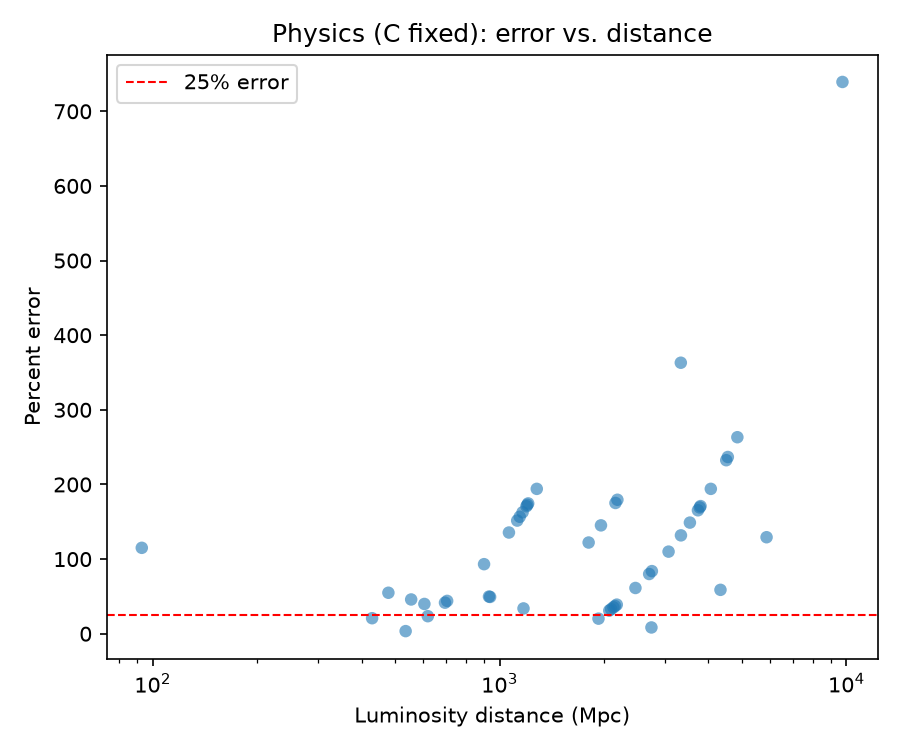
\includegraphics[width=0.75\textwidth]{figures/physics_uncalibrated_vs_distance.png}
\caption{Physics estimator, uncalibrated $C$: percent error vs. luminosity distance. Error rises sharply and consistently with distance.}
\label{fig:physics-uncal-dist}
\end{figure}

\begin{figure}[H]
\centering
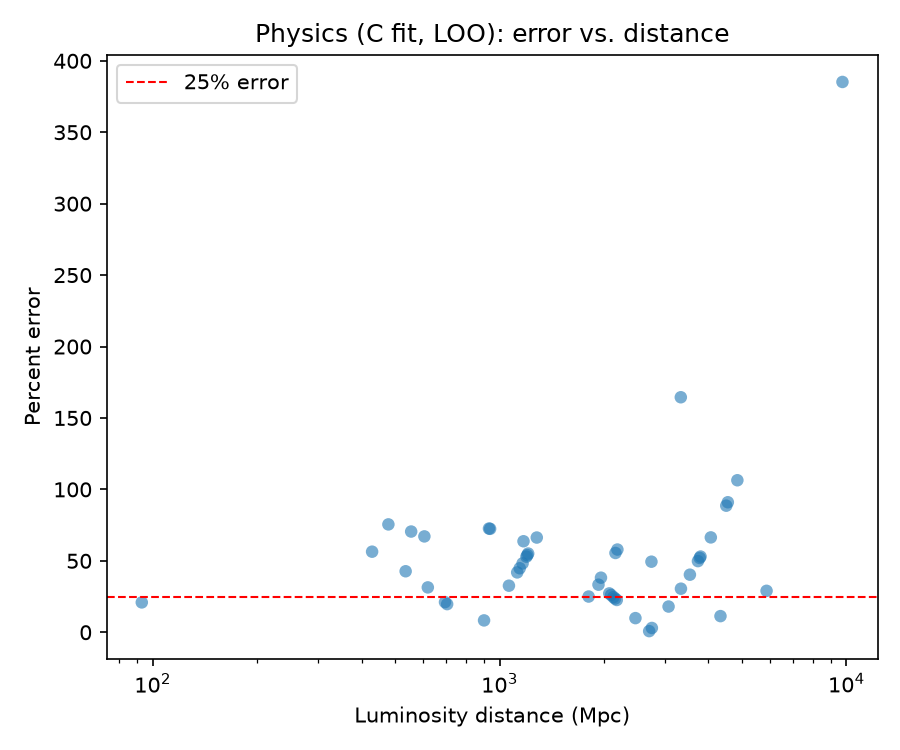
\includegraphics[width=0.75\textwidth]{figures/physics_calibrated_vs_distance.png}
\caption{Physics estimator, $C$ properly fit (leave-one-out): percent error vs. luminosity distance. The same rising trend survives calibration, at a compressed scale.}
\label{fig:physics-cal-dist}
\end{figure}

\subsection{The Trivial Baseline Finding}

A source-class-midpoint baseline -- no distance, no fitting, no per-event information beyond the classification label -- achieves a 47\% within-$\pm25\%$ rate and a 47\% bin-hit rate, both close to (and on the $\pm25\%$ metric, better than) the distance-only statistical model's 35\%/51\%. The initial explanation for this (that distance and source class are correlated, since heavier \gls{bbh} systems are both louder and visible further out) does not hold up: the 49-event validation set is 48/49 (98\%) \gls{bbh}, with only one unclassified event and zero \gls{bns}/\gls{nsbh}. There is essentially no class diversity in this sample to correlate distance against. The baseline's competitiveness more plausibly reflects that guessing near the sample's dominant, modal value is a strong strategy when the sample is this concentrated -- not evidence of a genuine distance-class relationship. The population-average baseline, by contrast, is uniformly poor (0\% within $\pm25\%$), confirming that per-event structure of \emph{some} kind is genuinely needed. Whether class adds signal beyond distance specifically could not be established on this 49-event sample -- but is resolved directly in Section~\ref{sec:catalog-validation} using the catalog-backed set's real class diversity.

\begin{figure}[H]
\centering
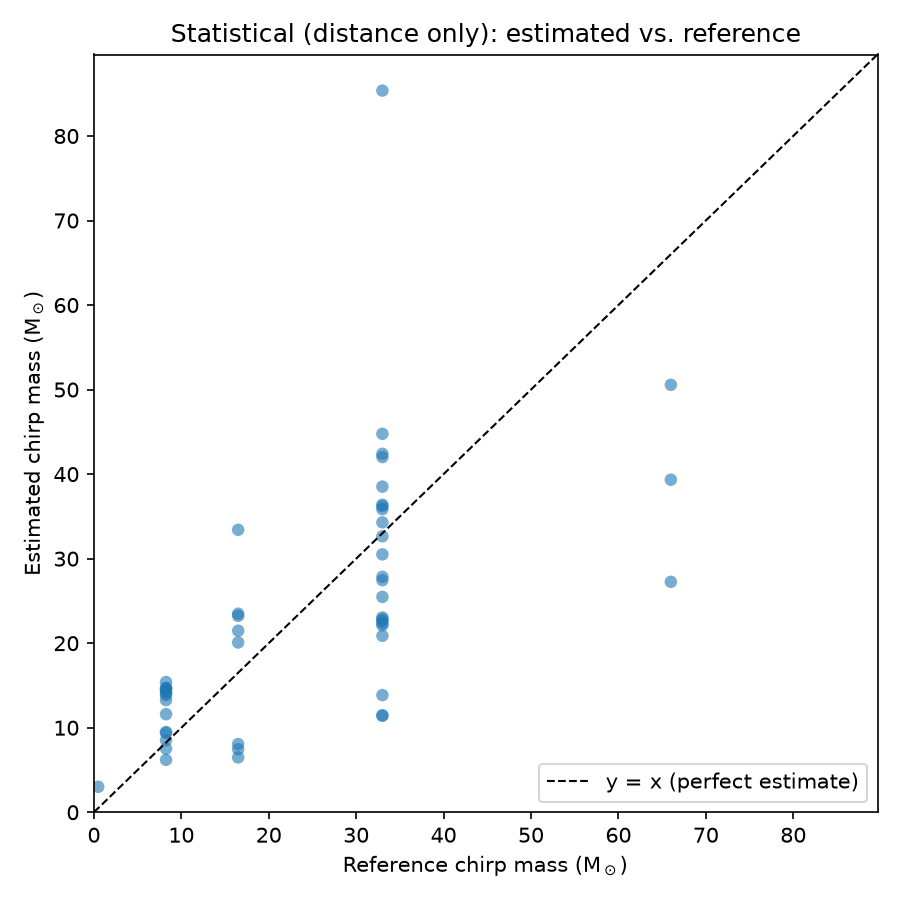
\includegraphics[width=0.75\textwidth]{figures/statistical_scatter.png}
\caption{Statistical estimator: estimated vs. reference chirp mass. The vertical banding reflects the reference values themselves being quantized into LVK's discrete mass bins (midpoints at 8.25, 16.5, 33, 66 M$_\odot$), not continuous measurements.}
\label{fig:statistical-scatter}
\end{figure}

\subsection{Decision-Gate Classification}

Following the project's decision-gate taxonomy (\texttt{validated\_approximation} $\mid$ \texttt{useful\_constraint} $\mid$ \texttt{exploratory\_only} $\mid$ \texttt{unsupported}):

\begin{itemize}
    \item \textbf{Physics (SNR-scaling) estimator, circular-only inputs: \texttt{unsupported}.} Fails even after properly fitting its calibration constant, with a systematic, physically-explained bias that no calibration choice removes -- because the one input it depends on most (\gls{snr}) is structurally absent from circular text. Section~\ref{sec:catalog-validation}'s catalog validation clarifies the scope of this: the formula itself is not unsupported in the abstract (given real \gls{snr}, it more than halves its own error), only as a circular-derived estimator specifically. Era-specific calibration (O3 vs.\ O4) closes a further, smaller slice of that gap (31.5\%$\to$26.6\%, Section~\ref{sec:catalog-validation}), but SNR remains the dominant lever by a wide margin.
    \item \textbf{Statistical (distance-only) estimator: \texttt{useful\_constraint}.} Not a validated per-event measurement, but a real, reproducible signal (best \gls{mae} and bin-hit rate of any method tested) useful for narrowing the plausible mass range. On the small circular-only set, a zero-fitting class-based baseline looked competitive, raising the question of whether distance was an independently powerful signal or just correlated with class; the larger catalog-backed set answers this directly (Section~\ref{sec:catalog-validation}) -- distance alone outperforms class alone and combining the two does not improve on distance alone, so the signal is genuinely distance's, not borrowed from classification.
\end{itemize}

\section{AI-Model Comparison Study}

% TODO: this section is a placeholder pending the fresh comparison batch
% planned for Days 6-7 of the sprint. Initial (~50-event) results using a
% structured Role/Task/Context/Reasoning/Output/Stopping prompting framework
% across five free-tier LLMs (ChatGPT, Gemini, Claude, DeepSeek, Grok) showed
% inconsistent reliability -- some models correctly identified non-BBH events
% and cited catalogs cleanly, others gave partial or unverifiable answers
% from memory alone. Full results and analysis to be added here.

\section{GW Pathfinder Evaluation}

% TODO: pending the minimal prototype build (sprint Days 8-10). This section
% will report the M9.4 test-question evaluation (factual retrieval,
% comparison, filtering, out-of-scope categories) once the prototype exists.

\chapter{Conclusion and Recommendation}
\label{ch:conclusion}

\section{Summary of Findings}

This project set out to determine whether \gls{gcn} circular text alone can support a fast, approximate chirp-mass estimate. The answer, established with evidence rather than assumed: not reliably with the standard \gls{snr}-scaling physics formula, because network \gls{snr} and orbital inclination are structurally absent from circular text -- confirmed both by a data-availability audit and by the formula's failure even after properly calibrating its one free constant (Chapter~\ref{ch:results}). A statistical alternative based on distance alone performs meaningfully better, though a trivial classification-based baseline tempers how much of that improvement is genuinely new information.

\section{Contribution}

The core contribution is not a proof that circular-level chirp-mass estimation works well -- it does not, cleanly, and this report states that plainly. The contribution is: a reproducible, provenance-tracked pipeline converting unstructured circular text into a structured, auditable dataset; an honest, quantified feasibility result that explains \emph{why} the physics-motivated approach falls short and what a data-driven alternative achieves instead; and a literature-grounded case, backed by a direct comparison study, for why an AI-assisted tool in this domain should be built on retrieval rather than model memory.

\section{Limitations}

\begin{itemize}
    \item The validation set is small (49 events); leave-one-out cross-validation reduces, but does not eliminate, overfitting risk at this sample size.
    \item Reference-mass events are, by construction, drawn from later observing runs than O4a, since O4a circulars never report this field; O4a data contributed to the availability audit but no validation examples.
    \item The statistical model uses distance alone; \gls{far} and classification probability were tested as additional predictors and did not help at this sample size, though this may change as the archive accumulates more circulars with reference chirp mass.
    \item No external reference catalog (e.g. \gls{gwtc}/\gls{gwosc}) was incorporated, by scope decision; doing so was identified as a possible future extension pending supervisor guidance on scope.
\end{itemize}

\section{Recommendation}

Given the coarse, bin-quantized nature of the reference chirp mass values circulars do report, this project recommends that future work on this problem adopt ``predict the correct mass bin'' rather than a fixed percentage-error target as the primary success criterion, since the latter implicitly demands more precision than the ground truth itself provides.

\section{Future Work}

\begin{itemize}
    \item Expand the historical validation sample as more circulars with reference chirp mass accumulate, or by incorporating an external catalog if scope permits.
    \item Test whether source classification, more carefully combined with distance (rather than as a simple alternative baseline), improves on the current statistical estimator.
    \item Develop an uncertainty-aware estimator rather than a point estimate.
    \item Complete the AI-model comparison study on a larger, fresh event batch, and complete a working (not just designed) GW Pathfinder prototype.
    \item Explore additional circular-derivable parameters beyond chirp mass (e.g. sky localization, detector count, event time) not yet incorporated into the pipeline.
    \item Prepare a publication-quality version of the statistical analysis for the strongest result, per the project's longer-term research-paper goal.
\end{itemize}


\bibliographystyle{apacite}
\bibliography{references}

% \appendix
% \input{chapters/appendix}

\end{document}
